\documentclass[a4paper]{article}
\usepackage{float}
\usepackage{fullpage, amsmath, amssymb, verbatim} % Package to use full page
\usepackage{graphicx}
\usepackage{adjustbox}

\title{Deep Learning: Assignment Three}
\author{Aditi Nair (asn264) and Akash Shah (ass502)}
\date{May 2, 2017}
\begin{document}

\maketitle

\section{Generative Adversarial Networks}

\begin{enumerate}
\item{\textit{Explain generative modeling.} 
\newline
\newline
A generative model uses training data drawn from an unknown distribution $p$, and learns a representation of the distribution, called $\hat{p}$. Generative models can represent $\hat{p}$ directly, generate samples from $\hat{p}$, or both. 

}
\item{\textit{Compare Generative Adversarial Networks (GANs) with other Unsupervised learning approaches, such as Auto-encoders. Explain the difference.}
\newline
\newline
We can compare GANs with other models that estimate probability distributions by choosing distributions that maximize the likelihood of the observed training data. Within this category, we can distinguish between generative models that implicitly and explicitly represent the probability density function $\hat{p}$. 
\newline
\newline
For explicit density models, the maximum likelihood estimation (MLE) task involves choosing probability density functions for $\hat{p}$, and then using gradient descent methods to choose appropriately parametrize the density functions. Creating MLE-driven generative models that develop explicit density functions are challenging because effectively estimating probability distributions often requires complex models, whose optimization can be computationally intractable. Currently, this is addressed by carefully constructing tractable explicit density functions (like Fully Visible Belief Nets, or FVBNs) and by constructing intractable explicit density functions (like Variational Auto-encoders, or VAEs), which require approximations to complete the MLE task. We will focus on comparing FVBNs, VAEs and GANs since they are currently three of the most popular approaches to generative modeling.
\newline
\newline
FVBNs use the rule of conditional probabilities to represent a distribution $\hat{p} \left( \textbf{x} \right) $ over an $n$-dimensional vector $\textbf{x}$:
$$\hat{p} \left( \textbf{x} \right) = \prod_{i=1}^n \hat{p} \left( x_i | x_1,...x_{i-1} \right) $$
That is, the probability distribution over $\textbf{x}$ is defined as the product of the conditional probabilities over its individual components. In particular, this operation cannot be parallelized because of the conditional nature of the computation. In WaveNet, a popular approach to FVBNs, each $\hat{p} \left( x_i | x_1,...x_{i-1} \right)$ is computed by a neural network. Accordingly, the computation of each conditional probability can be expensive, and can only be executed sequentially, making it difficult to scale the model for more demanding tasks. 
\newline
\newline
Next, we consider VAEs, which fall in the category of explicit density models which rely on approximation to complete the MLE task. Intuitively, VAEs use encoders to transform high-dimensional input vectors $x$ into a lower-dimensional latent space representations $z$, and then attempt to re-construct the original vectors using decoder networks. Probabilistically, we can argue that we would like to calculate the posterior distribution $p \left(z|x \right) $ so that we have good estimates for $z$ given the training data $x$. In variational inference, we approximate this distribution with $\hat{p} \left( z|x \right)$. In order to optimize our choice of $ \hat{p} \left(z|x \right)$ we would like to minimize the Kullback-Leibler divergence:
$$KL\left( \hat{p} \left(z|x \right) |  p \left( z|x \right) \right)  = \int_{x} \hat{p}(z|x) log \frac{\hat{p}(x|z) }{p(z|x ) } $$
$$ = \int_{x} \hat{p}(z| x) log \ \hat{p}(z |x)  - \hat{p}(z| x) log \ p(z|x )  $$
$$ = \mathrm{E}_{\hat{p}} [ log  \hat{p}(z |x) ] - \mathrm{E}_{\hat{p}} [ log \ p (z | x) ]  $$
By Bayes' Rule:
$$ p (z|x) = \frac{p(x,z)}{p(x)}$$
So we can write:
$$KL\left( \hat{p} \left(z|x \right) |  p \left( z|x \right) \right) = \mathrm{E}_{\hat{p}} [ log  \hat{p}(z |x) ] - \mathrm{E}_{\hat{p}} \Big[ log \ \frac{p(x,z)}{p(x)} \Big] $$
$$ =   \mathrm{E}_{\hat{p}} [ log\  \hat{p}(z |x) ] - \mathrm{E}_{\hat{p}} [ log \ p(x,z) ] + log \ p(x)$$
Clearly the term $log \ p(x)$ is intractable. Either we must know the distribution $p(x)$ - in which case we have already solved the problem of generative modeling - or we must compute it by marginalizing over $z$ - $\int_z p(x|z) p(z) dz$ - which is intractable since the space of all possible $z$ is large. However, we observe that by maximizing the following tractable expression:
$$\mathrm{E}_{\hat{p}} [ log \ p(x,z) ] - \mathrm{E}_{\hat{p}} [ log\  \hat{p}(z |x) ] $$
we minimize the KL-divergence as written above. Therefore, in the VAE setting, we choose to maximize the above expression, known as ELBO, instead. However, optimizing over the ELBO only provides a lower bound over the original KL-divergence, which has an added $log \ p(x)$ term. In addition, if we choose an inappropriate distribution for the prior or the posterior of $\hat{p}$, then we end up selecting $\hat{p}$ poorly. This is the primary weakness of VAE models, in addition to the lower quality of their generated samples.
\newline
\newline
Finally, we consider GANs. A GAN can be described as a game between two adversarial players, a generator $G$ with parameters $\theta^G$ and a discriminator $D$ with parameters $\theta^D$. The generator creates samples which appear to be drawn from original distribution $p$. The discriminator classifies samples as being real (drawn from the original distribution) or fake (created by the generator), and is trained to minimize the following loss:
$$ J^D(\theta^D, \theta^G) = -\frac{1}{2} \mathrm{E}_{x \sim p_{data}} [log\ D(x)] - \frac{1}{2} \mathrm{E}_z [log\ (1 - D(G(z)))]$$
The first summand expresses the cross-entropy loss of the discriminator on real samples drawn from the training data. $D(x)$ expresses the discriminator's probability estimate that $x$ is sampled from the data. If $D(x) = 1$, then $log\ D(x) = 0$ and the left summand is minimized. The second summand expresses the cross-entropy loss of the discriminator on ``fake" samples created by the generator. $z$ are noise vectors sampled from a prior distribution (e.g. a uniform distribution on a unit hyper-cube), which are fed to $G$ to create fake samples. $D(G(z))$ expresses the probability that $z$ is sampled from the data distribution, so $1- D(G(z))$ expresses the probability that $z$ is fake. If $D(G(z)) = 0$, then the discriminator is certain that a fake is indeed fake, and the right summand is minimized. Note that $ J^D(\theta^D, \theta^G)$ is a function of $\theta^D$ and $\theta^G$, but $D$ can only optimize over $\theta^D$.
\newline
\newline
Next, the generator is trained to ``fool" the discriminator. The loss function used for the generator can vary, but a common one is the cross-entropy loss:
$$J^G(\theta^G, \theta^D) = -\frac{1}{2} \mathrm{E}_z [log \ D(G(z))] $$
$J^G$ is a function of $\theta^D$ and $\theta^G$ but $G$ can only optimize over $\theta^G$. If $G(z)$ looks exactly like a sample drawn from $p_{data}$, then $D(G(z)) = 1$ and we will minimize $J^G$.
\newline
\newline
Typically, both the generator and the discriminator are neural networks which are trained simultaneously using gradient descent on real and fake samples. Unlike FVBNs and VAEs, GANs only provide us with an implicit representation of $\hat{p}$, since the generator is a neural network constructed to create the $G(z)$ samples. For the same reason, unlike FVBNs, GANs can generate an entire sample simultaneously. Whereas VAEs require you to carefully select the distribution for the approximator $\hat{p}$, the neural networks used in GANs are generally considered universal approximators. In addition, unlike (most) VAEs, a GAN trained with sufficient data can theoretically recover the true distribution $p_{data}$ - it is clear above that both $J^G$ and $J^D$ can be minimized directly, whereas we can only minimize the ELBO of the VAE loss function. Finally, it is worth noting that GANs are (subjectively) consider to produce better samples than VAEs and FVBNs.

\begin{comment}
Credit https://jaan.io/what-is-variational-autoencoder-vae-tutorial/ for VAE explanation
\end{comment}
}
\item{\textit{Explain conditional generation using GANs, versus the vanilla unconditional version. Please briefly draw a diagram when training conditional GANs, with the condition context C, generator G, discriminator D, random vector z and output x.}
\newline
\newline
In the previous presentation of GANs, we described ``vanilla" unconditional generation where we take $z$ samples from a noisy prior distribution and feed them into the generator $G$. One problem is that we have no control over the kind of sample we generate - or, mathematically speaking, on the distribution of the samples being generated. 
\newline
\newline
To address this issue, Mirza and Osindero (2014) suggest building Conditional GANs, which condition both the generator and discriminator on some context $C$. For example, Mirza and Osindero set $C$ as one-hot vectors indicating class labels for data.
\newline
\newline
In the generator, we combine the noise vector $z$ with the context $C$ at the input layer (for example, by concatenation), before feeding it through an appropriately-sized convolutional network to generate $G(z|C)$. Ideally, $G(z|C)$ should look like it belongs to the class of $C$. In the discriminator, we similarly combine the inputs $X$ (either $G(z|C)$ or $x \sim p_{data}$) with the appropriate one-hot vector $C$ before feeding it through an appropriately-sized convolutional network to compute $D(X|C)$. Finally, to generate samples of a specific class, we simply sample $z$ from the noise prior, concatenate with the $C$ vector for the intended class and compute $G(z|C)$. 
\newline
\newline
Below, we provide a diagram of the Conditional GAN framework (borrowed from Mirza and Osindero and modified with our notation):
\begin{figure}[H]
  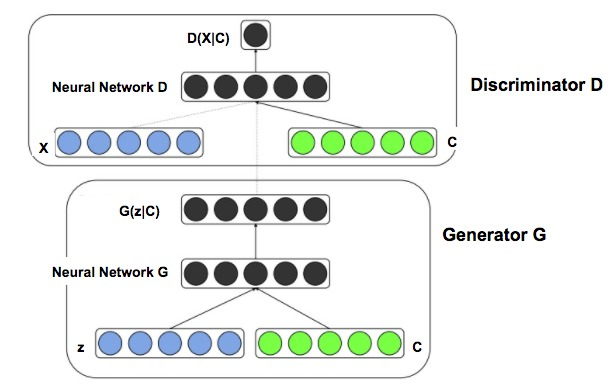
\includegraphics[scale=3]{images/my_conditional_gan.jpg}
  \label{fig:boat1}
\end{figure}

\begin{comment}
Cite: Mirza and Osindero "Conditional Generative Adversarial Networks" (2014)
\end{comment}

}
\end{enumerate}

\section{GAN Workhouse}


\end{document}
